%%%%%%%%%%%%%%%%%%%%%%%%%%%%%%%%%%%%%%%%%%%%%%%%%%%%%%%%%%%%%%%%%%%%%%%%%%
%% Review Volume (last updated on 20-4-2015)                            %%
%% Trim Size: 9in x 6in                                                 %%
%% Text Area: 7.35in (include runningheads) x 4.5in                     %%
%% Main Text: 10 on 13pt                                                %%
%% For support: Yolande Koh, <ykoh@wspc.com.sg>                         %%
%%              D. Rajesh Babu, <rajesh@wspc.com.sg>                    %%
%%%%%%%%%%%%%%%%%%%%%%%%%%%%%%%%%%%%%%%%%%%%%%%%%%%%%%%%%%%%%%%%%%%%%%%%%%
%%
%\documentclass[wsdraft]{ws-rv9x6} % to draw border line around text area
\documentclass{ws-rv9x6}
\usepackage{subfigure}   % required only when side-by-side / subfigures are used
\usepackage{ws-rv-thm}   % comment this line when `amsthm / theorem / ntheorem` package is used
\usepackage{ws-rv-van}   % numbered citation & references (default)
%\usepackage{ws-index}   % to produce multiple indexes
\makeindex
%\newindex{aindx}{adx}{and}{Author Index}       % author index
%\renewindex{default}{idx}{ind}{Subject Index}  % subject index

\begin{document}

\chapter[Using World Scientific's Review Volume Document Style]{Using World Scientific's Review Volume\\ Document Style}\label{ra_ch1}

\author[F. Author and S. Author]{First Author and Second Author\footnote{Author footnote.}}
%\index[aindx]{Author, F.} % or \aindx{Author, F.}
%\index[aindx]{Author, S.} % or \aindx{Author, S.}

\address{World Scientific Publishing Co, Production Department,\\
5 Toh Tuck Link, Singapore 596224, \\
f\_author@wspc.com.sg\footnote{Affiliation footnote.}}

\begin{abstract}
The abstract should summarize the context, content and conclusions of
the paper in less than 200 words. It should not contain any references
or displayed equations. Typeset the abstract in 9 pt Times roman with
baselineskip of 11 pt, making an indentation of 1.5 pica on the left
and right margins.
\end{abstract}
%\markright{Customized Running Head for Odd Page} % default is Chapter Title.
\body

%\tableofcontents

\section{Using Other Packages}\label{ra_sec1}
The WSPC class file has already loaded the packages \verb|amsfonts,|
\verb|amsmath, amssymb, graphicx, rotating| and \verb|url| at the
startup. \verb|Check.tex| is an utility to test for all the files
required by World Scientific review volume project are available in
your present \LaTeX\ installation.

{\bf Usage:} \verb|latex check.tex|

Please try to limit your use of additional packages. They frequently
introduce incompatibilities. This problem is not specific to the
WSPC styles, it is a general \LaTeX{} problem. Check this manual
whether the required functionality is already provided by the WSPC
class file. If you do need third-party packages, send them along
with the paper. In general, you should use standard \LaTeX{}
commands as much as possible.

\section{Layout}
In order to facilitate our processing of your article, please give
easily identifiable structure to the various parts of the text by
making use of the usual \LaTeX{} commands or by your own commands
defined in the preamble, rather than by using explicit layout
commands, such as \verb|\hspace, \vspace, \large|,
etc. Also, do not redefine the page-layout parameters. For more
information on layout and font please refer
\url{http://www.worldscientific.com/sda/1020/rv-instruction9x6_2e.pdf}.

\subsection{Input used to produce a chapter}
\begin{verbatim}
\documentclass{ws-rv9x6}
%\usepackage{subfigure}% to produce side-by-side / subfigures
\usepackage{ws-rv-thm}% comment when other thm package is used
\usepackage{ws-rv-van}% default - numbered citation/references
%\usepackage{ws-index}% to produce multiple indexes
\makeindex
%\newindex{aindx}{adx}{and}{Author Index}      % author index
%\renewindex{default}{idx}{ind}{Subject Index} % subject index
\begin{document}
\chapter[Short Title]{Full Title}
\author[F. Author]{First Author}
%\aindx{Author, F.}                       % author index entry
\address{World Scientific Publishing...}
\begin{abstract}
The abstract should ...
\end{abstract}
\body
\section{Using Other Packages}
The class file has...
\begin{appendix}[Optional Appendix Title]
\section{Sample Appendix}
Text...
\end{appendix}
%\begin{thebibliography}{9}        % for non BIBTeX users
%\bibitem{ams04} \AmS, \emph{\AmS-\LaTeX{} ...
%\end{thebibliography}
\bibliographystyle{ws-rv-van}
\bibliography{ws-rv-sample}
%\printindex[aindx]                % to print author index
\printindex
\end{document}
\end{verbatim}

\section{Using ws-rv9x6}
You can obtain these files from our web pages at:

\begin{itemlist}
\item \url{http://www.worldscientific.com/page/authors/review-style} and
\item \url{http://www.icpress.co.uk/authors/stylefiles.shtml#review}.
\end{itemlist}

\subsection{Class options and extra packages}
The class file, \verb|ws-rv9x6.cls| provides the following options:
\begin{alphlist}[onethmnum]
\item [\tt wsdraft] To draw border line around text area.\\
Default: no border line around text area.
\item[\tt addchapnum] Appends chapter number, e.g. 1.1. Section, Theorem 1.1., Table 1.1., etc\\
Default: 1. Section, Theorem 1., Table 1., etc.,
\item[\tt onethmnum] To number all theorem-like objects in a
single sequence, e.g. Theorem~1., Definition 2., Lemma 3., etc.\\
Default: individual numbering on different theorem-like objects,
e.g. Theorem 1., Definition 1., Lemma 1., etc.\\
\verb|ws-rv-thm| package is required.
\end{alphlist}

Apart from the packages mentioned in Sec~\ref{ra_sec1}, the WSPC
class also requires the following in-house packages for customizing
the theorems, citations and references.\\[6pt]

\noindent
{\tablefont
\begin{tabular}{@{}ll@{}}
{\bf Vancouver (numbered)}\\
\quad\verb|\usepackage{ws-rv-van}| & -- Superscript$^1$ (Default style)\\
\quad\verb|\usepackage[square]{ws-rv-van}| & -- Bracketed [1]\\[6pt]
{\bf Harvard (author-date)}\\
\quad\verb|\usepackage{ws-rv-har}| & -- (Author, 1994)
\end{tabular}\\[6pt]}

\noindent{\bf The contributors are advised to consult the managing editor for the chosen option (e.g., \verb|ws-rv-har|, \verb|addchapnum|, \verb|onethmnum|).}

\section{User Defined Macros}
User defined macros should be placed in the preamble of the article, and not at any other place in the document. Such private definitions, i.e. definitions made using the commands \verb|\newcommand, \renewcommand|, \verb|\newenvironment| or \verb|\renewenvironment|, should be used with great care. Sensible, restricted usage of private definitions is encouraged. Large macro packages and Definitions that are not used in the article should be avoided. Do not change existing environments, commands and other standard parts of \LaTeX.

\section{Running Head}\index{running head}

The WSPC prefers ``Author Name(s)'' as even page header and ``Chapter Title'' as odd page header.

\begin{table}[ht]
\tbl{This table shows how the author names should appear in the
running head and TOC depending upon the number of authors
contributing that paper.} {\begin{tabular}{@{}ll@{}} \toprule
No. of Authors & Author Names\\
\colrule
1 & L. Hatcher\\
2 & I. A. Pedrosa \& I. Guedes\\
3 & B. Feng, X. Gong \& X. Wang\\
4 and more & S. R. Choudhury {\it et al.}\\\botrule
\end{tabular}}
\begin{tabnote}
For TOC and Running Heads, the author names should appear in initial
and surname format, e.g. Lee Hatcher should be abbreviated as
L.~Hatcher.
\end{tabnote}\label{ra_tbl1}
\end{table}

Running heads are obtained by the arguments supplied in the square
brackets of \verb|\chapter[#1]{#2}| and \verb|\author[#1]{#2}|
commands, e.g.,
\begin{verbatim}
\chapter[Short Title for Running Head]{Full title}
\author[F. Author and S. Author]
       {First Author and Second Author}
\end{verbatim}

When more than one \verb|\author| command is used, the names are
combined and included as the last \verb|\author|'s argument, e.g.,

\begin{verbatim}
\chapter[Short Title for Running Head]{Full title}
\author{First Author}
\address{First author's address}
\author[F. Author and S. Author]{Second Author}
\address{Second author's address}
\end{verbatim}

\section{Chapters}
Each chapter should normally be in a separate file. The chapter
title is typeset by using the \verb|\chapter[#1]{#2}| command, where
\verb|[#1]| is an optional short title to be used as a running head
if the title is too long and \verb|#2| is the full title of the
chapter. The short, edited version of the title appears in the table
of contents and running head. The chapter title should be typed in a
way such that only the initial character is in upper case and the
rest is in lower case.

\section{Sectional Units}
Sectional units are obtained in the usual way, i.e. with the \LaTeX{}
instructions \verb|\section|, \verb|\subsection|,
\verb|\subsubsection|, and \verb|\paragraph|.

\section{Section}
Text...

\subsection{Subsection}
Text...

\subsubsection{Subsubsection}
Text...

\paragraph{Paragraph}
Text...

\section*{Unnumbered Section}
Unnumbered sections can be obtained by \verb|\section*|.

\section{Lists of Items}\index{lists}
Lists are broadly classified into four major categories that can
randomly be used as desired by the author:
\begin{alphlist}[(d)]
\item Numbered list.
\item Lettered list.
\item Unnumbered list.
\item Bulleted list.
\end{alphlist}

\subsection{Numbered and lettered list}\index{lists!numbered and lettered}

\begin{enumerate}
\item The \verb|\begin{arabiclist}[]| command is used for the arabic
number list (arabic numbers appearing within or without parenthesis), e.g., (1),
(2); 1., 2. etc.\index{lists!numbered and lettered!arabic (1, 2, 3...)}

\smallskip

\item The \verb|\begin{romanlist}[]| command is used for the roman
number list (roman numbers appearing within parenthesis), e.g., (i),
(ii), etc.\index{lists!numbered and lettered!roman (i, ii, iii...)}

\smallskip

\item The \verb|\begin{Romanlist}[]| command is used for the capital roman
\hbox{number list} (capital roman numbers appearing within parenthesis),
e.g., (I), (II), etc.\index{lists!numbered and lettered!Roman (I, II, III...)}

\smallskip

\item The \verb|\begin{alphlist}[]| command is used for the alphabetical
list (alphabetical characters appearing within parenthesis),
e.g., (a), (b), etc.\index{lists!numbered and lettered!alphabetical (a, b, c...)}

\smallskip

\item The \verb|\begin{Alphlist}[]| command is used for the capital
alphabetical list (capital alphabetical characters appearing within
parenthesis), e.g., (A), (B), etc.\index{lists!numbered and lettered!Alphabetical (A, B, C...)}
\end{enumerate}
Note: For all the above mentioned lists, it is obligatory to enter the last entry's number
in the list within the square bracket, to enable unit alignment.

Items numbered with lowercase Roman numerals:
\begin{romanlist}[(iv)]
\item item one
\item item two
    \begin{alphlist}[(d)]
    \item subitem one
    \item lists within lists can be numbered with lowercase alphabets
    \end{alphlist}
\item item three.
\end{romanlist}

\subsection{Bulleted and unnumbered list}\index{lists!bulleted and unnumbered}

\begin{itemlist}
\item The \verb|\begin{itemlist}| command is used for the bulleted list.

\smallskip

\item The \verb|\begin{unnumlist}| command is used for creating the
  unnumbered list with the turnovers hangindent by 1\,pica.
\end{itemlist}

Lists may be laid out with each item marked by a dot:
\begin{itemlist}
\item item one
\item item two
\begin{itemlist}
\item subitem one
\item subitem two
\item subitem three
\item subitem four.
\end{itemlist}
\item item three
\item item four
\item item five.
\end{itemlist}

\section{Theorems and Definitions}\index{theorems}
The WSPC document styles contain a set of pre-defined
environments for theorems, definitions, proofs, remarks etc.

All theorem-like objects use individual numbering scheme by default.
To number them in a single sequence, load the option
\verb|onethmnum| in the preamble., e.g.,
\verb|\usepackage[onethmnum]{ws-rv-thm}|.

\begin{verbatim}
\begin{theorem}
We have $\# H^2 (M \supset N) < \infty$ for an inclusion ...
\label{ra_thm1}
\end{theorem}
\end{verbatim}

\noindent produces

\begin{theorem}
We have $\# H^2 (M \supset N) < \infty$ for an inclusion $M \supset
N$ of factors of finite index.\label{ra_thm1}
\end{theorem}

\begin{verbatim}
\begin{theorem}[Longo, 1998]
For a given $Q$-system...
\[
N = \{x \in N; T x = \gamma (x) T, T x^* = \gamma (x^*) T\}\,,
\]
and $E_\Xi (\cdot) = T^* \gamma (\cdot) T$ gives ...
\label{ra_thm2}
\end{theorem}
\end{verbatim}

\noindent generates

\begin{theorem}[Longo, 1998]
For a given $Q$-system...
\[
N = \{x \in N; T x = \gamma (x) T, T x^* = \gamma (x^*) T\}\,,
\]
and $E_\Xi (\cdot) = T^* \gamma (\cdot) T$ gives a conditional
expectation onto $N$.
\label{ra_thm2}
\end{theorem}

The following environments are available by default with WSPC
document styles:

\begin{center}
{\tablefont
\begin{tabular}{ll}
\toprule Environment & Heading\\\colrule
\verb|algorithm| & Algorithm\\
\verb|answer| & Answer\\
\verb|assertion| & Assertion\\
\verb|assumption| & Assumption\\
\verb|case| & Case\\
\verb|claim| & Claim\\
\verb|comment| & Comment\\
\verb|condition| & Condition\\
\verb|conjecture| & Conjecture\\
\verb|convention| & Convention\\
\verb|corollary| & Corollary\\
\verb|criterion| & Criterion\\
\verb|definition| & Definition\\
\verb|example| & Example\\
\verb|lemma| & Lemma\\
\verb|notation| & Notation\\
\verb|note| & Note\\
\verb|observation| & Observation\\
\verb|problem| & Problem\\
\verb|proposition| & Proposition\\
\verb|question| & Question\\
\verb|remark| & Remark\\
\verb|solution| & Solution\\
\verb|step| & Step\\
\verb|summary| & Summary\\
\verb|theorem| & Theorem\\\botrule
\end{tabular}}\label{ra_theo}
\end{center}

\LaTeX{} provides \verb|\newtheorem| to create new theorem
environments. To add a new theorem-type environments to a chapter, use

\begin{verbatim}
\newtheorem{example}{Example}[section]
\let\Examplefont\upshape
\def\Exampleheadfont{\bfseries}
\end{verbatim}

\subsection{Proofs}
The WSPC document styles also provide a predefined proof environment for proofs.
The proof environment produces the heading
`Proof' with \hbox{appropriate} spacing and punctuation. A `Q.E.D.' symbol, $\square$,
can be appended at the end of a proof with the command \verb|\qed|, e.g.,

\begin{verbatim}
\begin{proof}
This is to test.
\end{proof}
\end{verbatim}

\noindent produces

\begin{proof}
This is to test.
\end{proof}

The proof environment takes an argument in curly
braces, which allows you to substitute a different name for the standard
`Proof'. If you want to display, `Proof of Lemma', then write

\begin{verbatim}
\begin{proof}[Proof of Lemma]
This is to test.
\end{proof}
\end{verbatim}

\noindent produces

\begin{proof}[Proof of Lemma]
This is to test.
\end{proof}

\section{Mathematical Formulas}
\paragraph{Inline:}
For in-line formulas use \verb|\( ... \) or $ ... $|. Avoid
built-up constructions, for example fractions and matrices, in
in-line formulas. Fractions in inline can be typed with a solidus e.g. \verb|x+y/z=0|.
\index{equations!inline}

\paragraph{Display:}
For numbered display formulas use the displaymath environment
\index{equations!display}
\verb|\begin{equation} ...| \verb|\end{equation}|.

And for unnumbered display formula use
\verb|\[ ... \]|. For numbered displayed
one line formulas always use the equation environment. Do not use
\verb|$$ ... $$|. For example, the input for:
\begin{equation}
\mu(n, t) = \frac{\sum\limits^\infty_{i=1}1
(d_i < t, N(d_i) = n)}
{\int\limits^t_{\sigma=0}1(N(\sigma)=n)d\sigma}\,.
\label{ra_eq1}
\end{equation}

\noindent is:

\begin{verbatim}
\begin{equation}
\mu(n, t)=\frac{\sum\limits^\infty_{i=1}1(d_i < t, N(d_i)=n)}
{\int\limits^t_{\sigma=0}1(N(\sigma)=n)d\sigma}\,.\label{ra_eq1}
\end{equation}
\end{verbatim}

For displayed multi-line formulas use the eqnarray environment.

\begin{verbatim}
\begin{eqnarray}
\zeta\mapsto\hat{\zeta}&=&a\zeta+b\eta\label{ra_eq2}\\
\eta\mapsto\hat{\eta}&=&c\zeta+d\eta\label{ra_eq3}
\end{eqnarray}
\end{verbatim}

\noindent\begin{eqnarray}
\zeta\mapsto\hat{\zeta}&=&a\zeta+b\eta\label{ra_eq2}\\
\eta\mapsto\hat{\eta}&=&c\zeta+d\eta\label{ra_eq3}
\end{eqnarray}

Superscripts and subscripts that are words or abbreviations, as in
\( \pi_{\mathrm{low}} \), should be typed as roman letters; this is
done as \verb|\( \pi_{\mathrm{low}} \)| instead of \( \pi_{low} \)
done by \verb|\( \pi_{low} \)|.

For geometric functions, e.g. exp, sin, cos, tan, etc. please use the macros
\verb|\sin, \cos, \tan|. These macros gives proper spacing in mathematical formulas.

It is also possible to use the \AmS-\LaTeX{}
package,\cite{ams04} which can be obtained from the \AmS, from various \TeX{}
archives.

\section{Floats}\index{floats}
\subsection{Tables}\index{floats!tables}
Put the tables and figures in the text with the table and figure environments,
and position them near the first reference of the table or figure in
the text. Please avoid long caption texts in figures and tables.
Do not put them at the end of the article.

\begin{verbatim}
\begin{table}[ht]
\tbl{Sample table caption.}
{\begin{tabular}{@{}cccc@{}} \toprule
Piston mass$^{\text a}$ & Analytical ...\\
& (Rad/s) & (Rad/s) \\ \colrule
1.0... \\
0.001...\\ \botrule
\end{tabular}}
\begin{tabnote}
$^{\text a}$Sample table footnote.
\end{tabnote}
\label{ra_tbl2}
\end{table}
\end{verbatim}

\begin{table}[ht]
\tbl{Sample table caption.}
{\begin{tabular}{@{}cccc@{}} \toprule
Piston mass$^{\text a}$ & Analytical frequency & TRIA6-$S_1$ model & \% Error \\
& (Rad/s) & (Rad/s) \\ \colrule
1.000 & \hphantom{0}281.0 & \hphantom{0}280.81 & 0.07 \\
0.010 & 2441.0 & 2441.00 & 0.00 \\
0.001 & 4130.0 & 4129.30 & 0.16\\ \botrule
\end{tabular}
}
\begin{tabnote}
$^{\text a}$Sample table footnote.
\end{tabnote}
\label{ra_tbl2}
\end{table}

For most tables, the horizontal rules are obtained by:
\begin{description}\index{floats!tables!rules}
\item[toprule] one rule at the top
\item[colrule] one rule separating column heads from data cells
\item[botrule] one bottom rule
\item[Hline] one thick rule at the top and bottom of the tables with multiple column heads
\end{description}

To avoid the rules sticking out at either end
of the table add \verb|@{}| before the first and after the last descriptors, e.g.
{@{}llll@{}}. Please avoid vertical rules in tables. But if you think the vertical rule is must,
you can use the standard \LaTeX{} \verb|tabular| environment.

By using \verb|\tbl| command in table environment, long captions will
be justified to the table width while the short or single line captions
are centered. \verb|\tbl{table caption}{tabular environment}|.
If we need the fixed width for
the tables, the command is \verb|\begin{tabular*}{#1}{@{}ll@{}}|
and \verb|\end{tabular*}|. In the argument \verb|#1| the width of
the table has to be given. For example if we need the table to be
of 25pc width, then the command is
\verb|\begin{tabular*}{25pc}{@{\extracolsep{fill}}ll@{}}|.

Headings which span for more than one column should be set using
\verb|\multicolumn{#1}{#2}{#3}| where \verb|#1| is the number of
columns to be spanned, \verb|#2| is the argument for the alignment
of the column head which may be either {c} --- for center
alignment; {l} --- for left alignment; or {r} --- for right
alignment, as desired by the users. Use {c} for column heads as
this is the WS style and \verb|#3| is the heading. A simplified
alternative version is \verb|\centre{#1}{#2}| where \verb|#1| is
the number of columns to be spanned and \verb|#2| the heading.
There should be a rule spanning the same columns below the
heading. Termed as spanner or bridge rule, it is generated using
the command \verb|\cline{n-m}| where \verb|n| is the number of the
first spanned column and \verb|m| that of the last spanned column.
\verb|\cline| should not be part of a row but follow immediately
after a \verb|\\|.

\def\p{\phantom{$-$}}
\def\pc{\phantom{,}}
\def\p0{\phantom{0}}
\begin{sidewaystable}
\tbl{Positive values of $X_0$ by eliminating $Q_0$ from Eqs.~(15)
and (16) for different values of the parameters $f_0$, $\lambda_0$
and $\alpha_0$ in various dimension.}
{\begin{tabular}{@{}ccccccccccc@{}}
\toprule\\[-6pt]
$f_0$ &$\lambda_0$ &$\alpha_0$
&\multicolumn{8}{c}{Positive roots ($X_0$)}\\[3pt]
\hline\\[-6pt]
&& &4D &5D &6D &7D &8D &10D &12D &16D\\[3.5pt]
\hline\\[-6pt]
\phantom{1}$-0.033$ &0.034 &\phantom{0}0.1\phantom{.01}
&6.75507,\p0 &4.32936,\p0 &3.15991,\p0 &2.44524,\p0
&1.92883,\p0 &0.669541, &--- &---\\[3.5pt]
&&&1.14476\pc\p0 &1.16321\pc\p0 &1.1879\pc\phantom{00}
&1.22434\pc\p0 &1.29065\pc\p0
&0.415056\pc\\[3.5pt]
\phantom{1}$-0.1$\phantom{33} &0.333 &\phantom{0}0.2\phantom{.01}
&3.15662,\p0 &1.72737,\p0 &--- &--- &--- &--- &--- &---\\[3.5pt]
&&&1.24003\pc\p0 &1.48602\pc\p0\\[3.5pt]
\phantom{1}$-0.301$ &0.302 &0.001
&2.07773,\p0 &--- &--- &--- &--- &--- &--- &---\\[3.5pt]
&&&1.65625\pc\p0\\[3.5pt]
\phantom{1}$-0.5$\phantom{01} &0.51\phantom{2} &\phantom{0}0.001
&--- &--- &--- &--- &--- &--- &--- &---\\[3.5pt]
$\phantom{1-}$0.1\phantom{01} &0.1\phantom{02}
&\phantom{0}2\phantom{.001} &1.667,\phantom{000} &1.1946\phantom{00,}
&--- &--- &--- &--- &--- &---\\[3.5pt]
&&&0.806578\pc &0.858211\pc\\[3.5pt]
$\phantom{1-}$0.1\phantom{01} &0.1\phantom{33} &10\phantom{.001}
&0.463679\pc &0.465426\pc &0.466489\pc &0.466499\pc
&0.464947\pc &0.45438\pc\p0 &0.429651\pc &0.35278\pc\\[3.5pt]
$\phantom{1-}$0.1\phantom{01} &1\phantom{.333}
&\phantom{0}0.2\phantom{01}
&--- &--- &--- &--- &--- &--- &--- &---\\[3.5pt]
$\phantom{-0}$1\phantom{.033} &0.001 &\phantom{0}2\phantom{.001}
&0.996033, &0.968869, &0.91379,\p0 &0.848544,&0.783787, &0.669541,
&0.577489, &---\\[3.5pt]
&&&0.414324\pc &0.41436\pc\p0 &0.414412\pc &0.414489\pc &0.414605\pc
&0.415056\pc &0.416214\pc\\[3.5pt]
\phantom{10}\phantom{.033} &0.001 &\phantom{0}0.2\phantom{01}
&0.316014, &0.309739, &--- &--- &--- &--- &--- &---\\[3.5pt]
&&&0.275327\pc &0.275856\pc\\[3.5pt]
\phantom{10}\phantom{.033} &0.1\phantom{33}
&\phantom{0}5\phantom{.001}
&0.089435\pc &0.089441\pc &0.089435\pc &0.089409\pc &0.08935\pc\p0
&0.089061\pc &0.088347\pc &0.084352\pc\\[3.5pt]
\phantom{10}\phantom{.033} &1\phantom{.333} &\phantom{0}3\phantom{.001}
&0.128192\pc &0.128966\pc &0.19718,\p0 &0.169063, &0.142103,
&--- &--- &---\\[3.5pt]
&&&& &0.41436\pc\p0 &0.414412\pc &0.414489\pc\\[3pt]
\Hline
\end{tabular}}\label{ra_tbl3}
\end{sidewaystable}

If a table contains note(s), as a
universal thumb-rule they should appear beneath the table set to its
width and seldom at the foot of the page. For the footnotes in the
table environment the command is
\verb|{\begin{tabnote}<text>\end{tabnote}}|. Appropriate symbols
should be included in the body of the table matching their
corresponding symbols in the footnotes where the footnotes are to be
placed immediately after the \verb|{\begin{tabnote}| command and
terminated before \verb|\end{tabnote}}\end{table}| command.

Landscape tables and figures can be typeset with following environments:
\begin{itemize}\index{floats!tables!landscape}
\item \verb|sidewaystable| and
\item \verb|sidewaysfigure|.
\end{itemize}

\noindent {\bf Example:}

\begin{verbatim}
\begin{sidewaystable}
\tbl{Positive values of ...}
{\begin{tabular}{@{}ccccccccccc@{}}
...
\end{tabular}} \label{ra_tbl3}
\end{sidewaystable}
\end{verbatim}

\subsection{Figures}\index{floats!figures}
The preferred graphics are tiff and Encapsulated
PostScript, eps in short, for any type of graphic. Our
\TeX\ installation requires eps, but we can easily convert tiff to eps.
Many other formats, e.g. pict (Macintosh), wmf (Windows) and various proprietary
formats, are not suitable. Even if we can read such files, there is no guarantee
that they will look the same on our systems as on yours.

Next adjust the scaling of the figure until it's correctly positioned,
and remove the declarations of the lines and any anomalous spacing.
If instead you wish to use some other method, then it's most
important to leave the right amount of vertical space in the figure
declaration to accommodate your figure. A figure is obtained with the following commands

\begin{verbatim}
\begin{figure}
\centerline{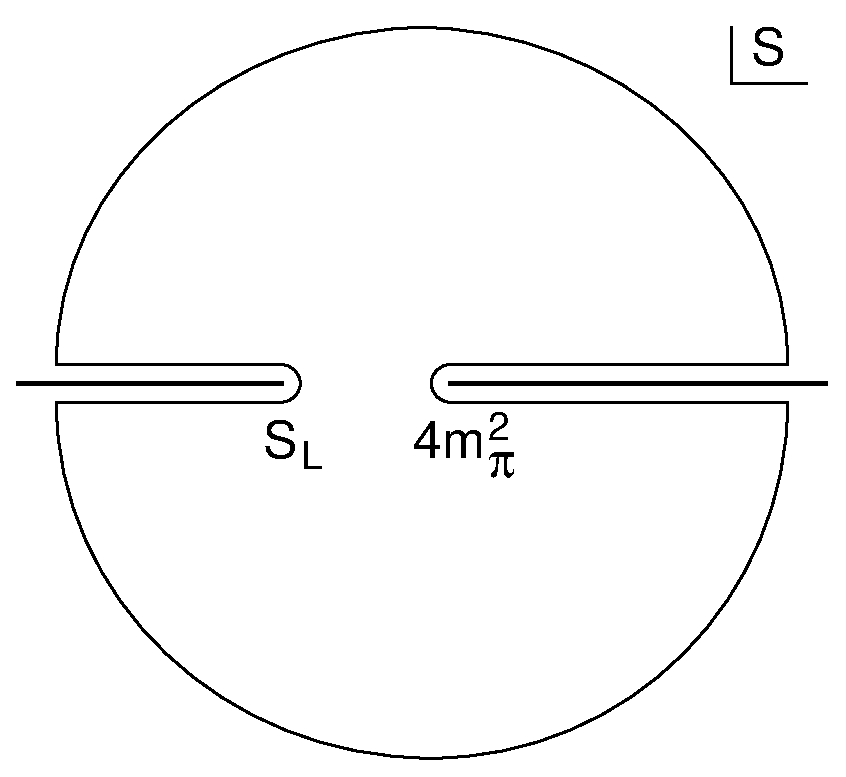
\includegraphics[width=3.8cm]{rv-fig1}}
\caption{Sample figure caption.} \label{ra_fig1}
\end{figure}
\end{verbatim}

\begin{figure}
\centerline{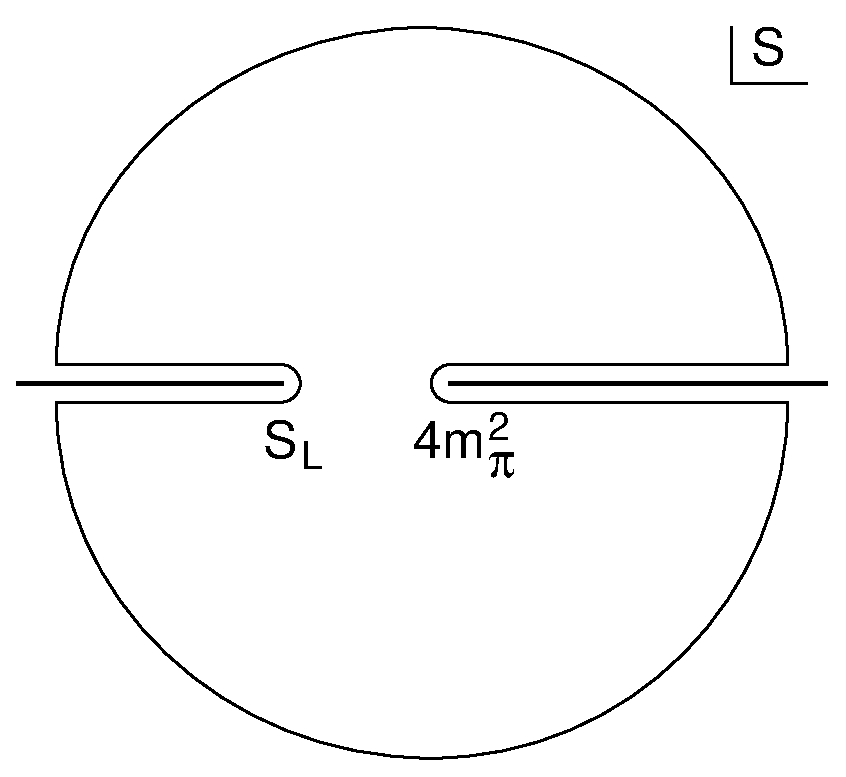
\includegraphics[width=3.8cm]{rv-fig1}}
\caption{Sample figure caption.}
\label{ra_fig1}
\end{figure}

Sub-figures are obtained with the following commands
\begin{verbatim}
\begin{figure}[ht]
\centerline{
  \subfigure[]
     {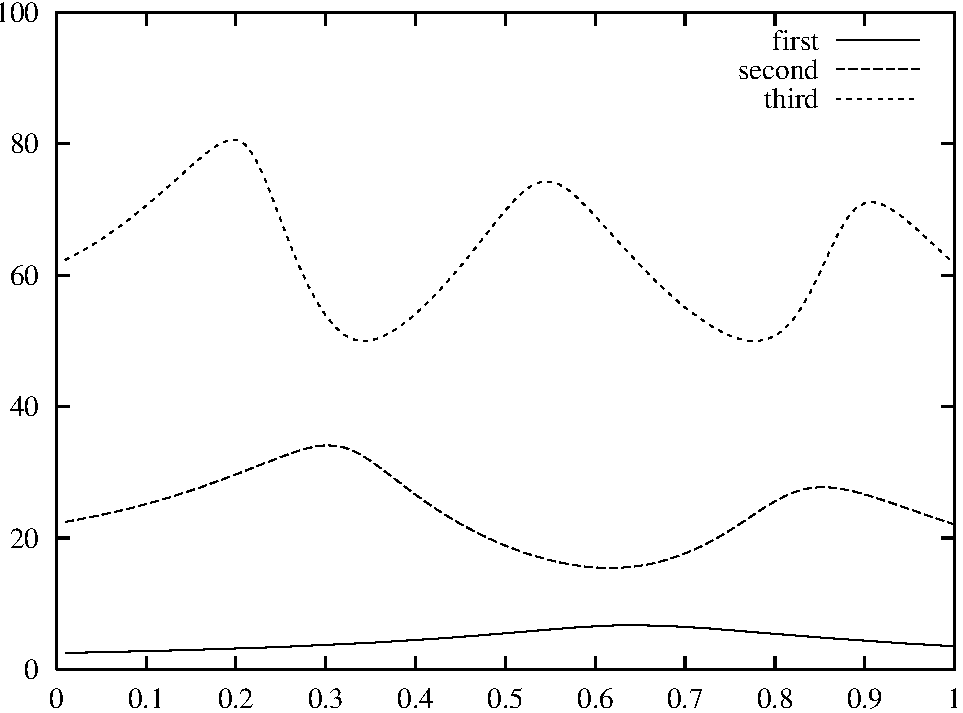
\includegraphics[width=2in]{rv-fig2a}\label{ra_fig2a}}
  \hspace*{4pt}
  \subfigure[Optional subcaption]
     {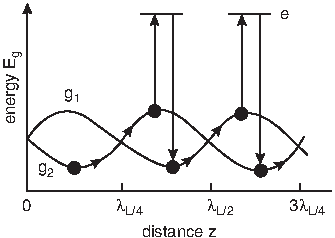
\includegraphics[width=2in]{rv-fig2b}\label{ra_fig2b}}
}
\caption{Common caption here.} \label{ra_fig2} % common label
\end{figure}
\end{verbatim}

\begin{figure}[ht]
\centerline{
  \subfigure[]
     {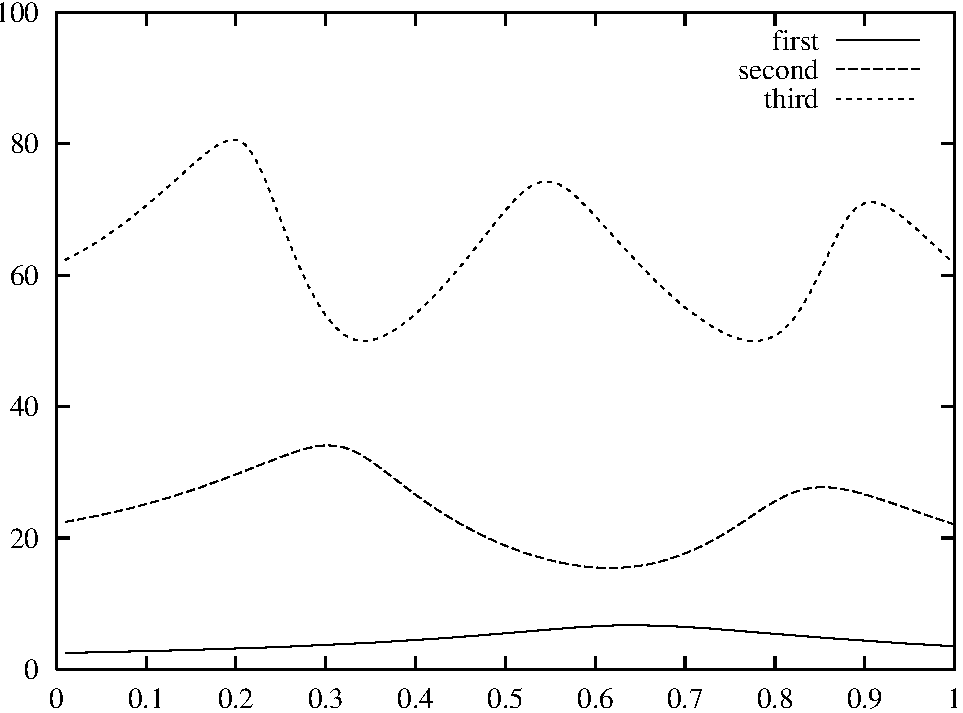
\includegraphics[width=2in]{rv-fig2a}\label{ra_fig2a}}
  \hspace*{4pt}
  \subfigure[Optional subcaption.]
     {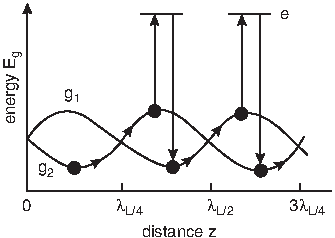
\includegraphics[width=2in]{rv-fig2b}\label{ra_fig2b}}
}
\caption{Common caption here.}\label{ra_fig2}
\end{figure}

Sub-figures \fref{ra_fig2a} and Fig.~\ref{ra_fig2b} are
referred with \verb|\fref{ra_fig2a}| and \verb|Fig.~\ref{ra_fig2b}| commands.

\begin{sidewaysfigure}
\centerline{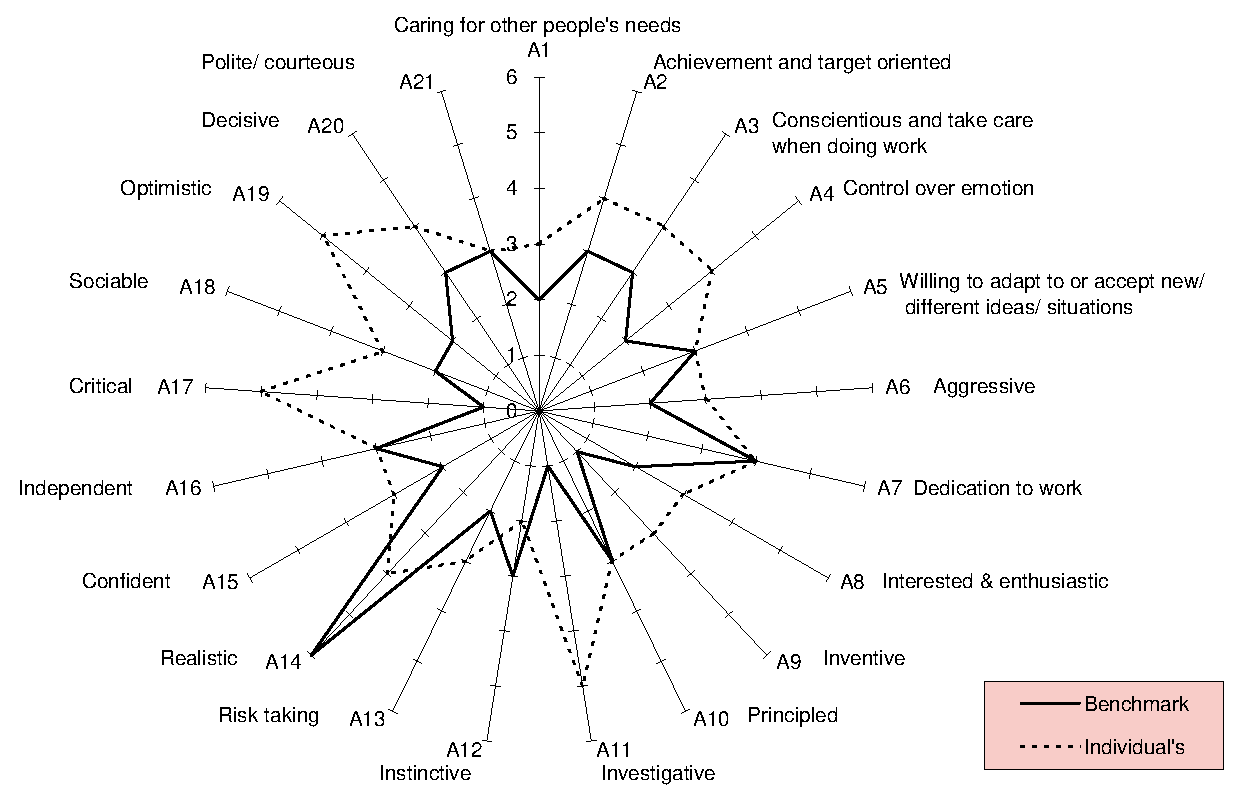
\includegraphics[width=6.6in]{rv-fig3}}
\caption{The bifurcating response curves of system
$\alpha=0.5$, $\beta=1.8$; $\delta=0.2$, $\gamma=0$:
(a) $\mu=-1.3$; and (b) $\mu=0.3$.}
\label{ra_fig3}
\end{sidewaysfigure}

Large figures and tables should be placed on a page by
themselves, e.g.,

\index{floats!figures!landscape}
\begin{verbatim}
\begin{sidewaysfigure}
\centerline{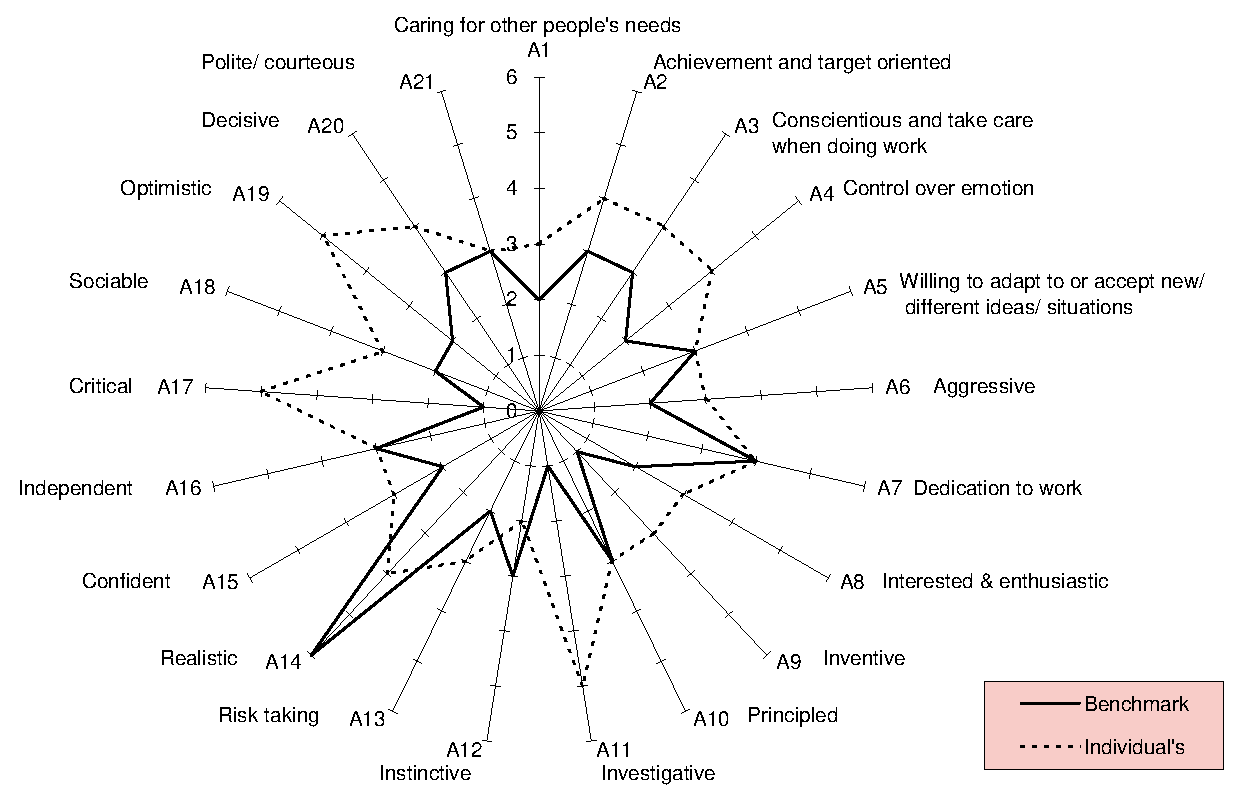
\includegraphics[width=6.6in]{rv-fig3}}
\caption{Sample figure caption.} \label{ra_fig3}
\end{sidewaysfigure}
\end{verbatim}

\begin{figure}[ht]
\centerline{
  \minifigure[Sample caption.]
     {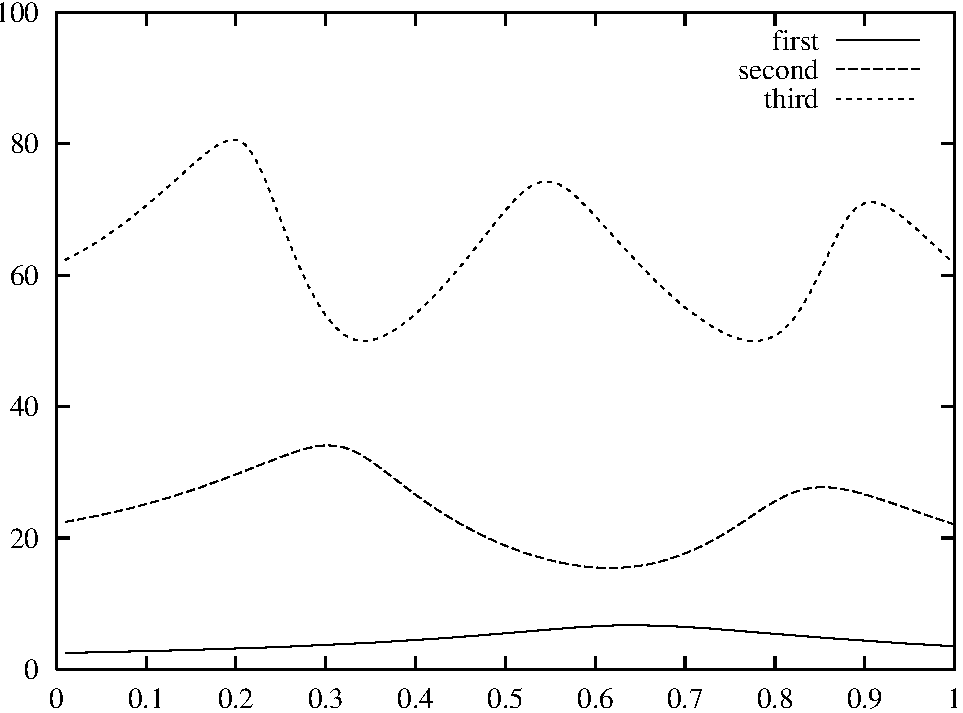
\includegraphics[width=2in]{rv-fig2a}\label{ra_fig4}}
  \hspace*{4pt}
  \minifigure[Sample caption.]
     {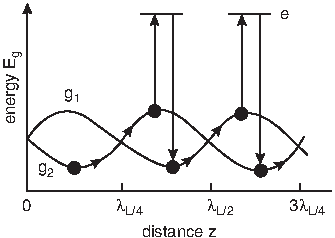
\includegraphics[width=2in]{rv-fig2b}\label{ra_fig5}}
}
\end{figure}

Side-by-side figures Fig.~\ref{ra_fig4} and \fref{ra_fig5} are
obtained with \verb|\minifigure| commands.

\begin{verbatim}
\begin{figure}[ht]
\centerline{
  \minifigure[Sample caption.]
     {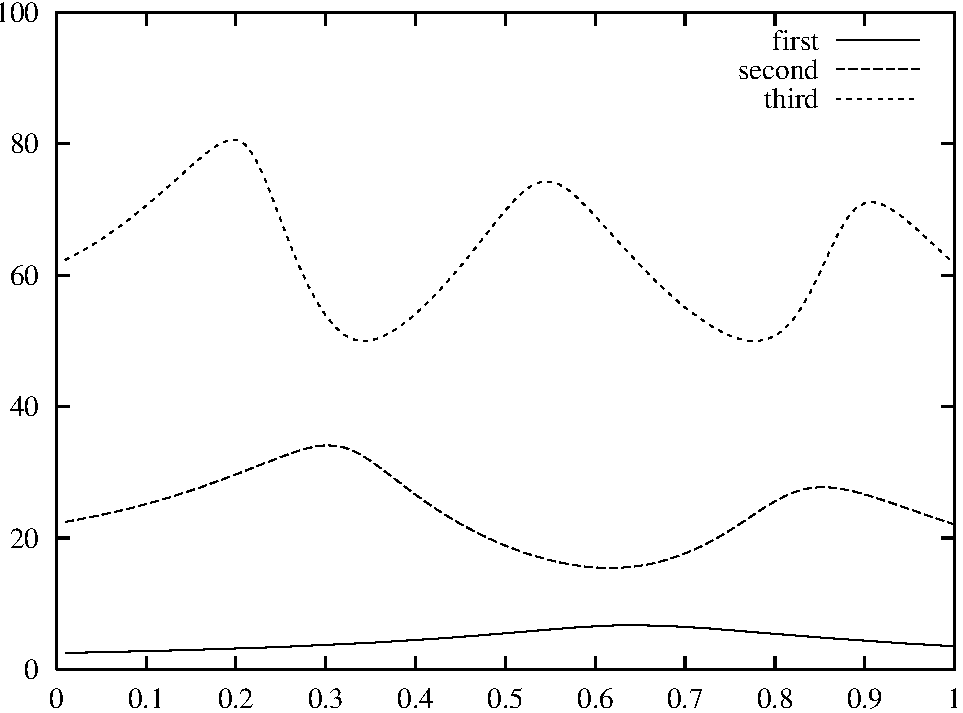
\includegraphics[width=2in]{rv-fig2a}\label{ra_fig4}}
  \hspace*{4pt}
  \minifigure[Sample caption.]
     {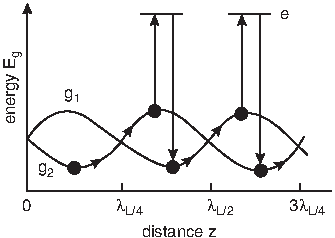
\includegraphics[width=2in]{rv-fig2b}\label{ra_fig5}}
}
\end{figure}
\end{verbatim}

\section{Cross-references}
Use \verb|\label| and \verb|\ref| for cross-references to
equations, figures, tables, sections, etc., instead
of plain numbers. Every numbered part to which one wants to refer,
should be labelled with the instruction \verb|\label|, for e.g.,

\begin{verbatim}
\begin{equation}
\mu(n, t)=\frac{\sum\limits^\infty_{i=1}1(d_i < t, N(d_i)=n)}
{\int\limits^t_{\sigma=0}1(N(\sigma)=n)d\sigma}. \label{ra_eq1}
\end{equation}
\end{verbatim}

With the instruction \verb|\ref| one can refer to a numbered part
that has been labelled, e.g., \verb|..., see also Eq. (\ref{ra_eq1})|.

\begin{center}{\tablefont
Some useful shortcut commands.
\begin{tabular}{lll}
\toprule
Shortcut & Equivalent & Output \\
command & \TeX\ command\\\colrule
\multicolumn{3}{@{}l}{In the middle of a sentence:}\\
\verb|\eref{ra_eq1}|  & Eq.~(\verb|\ref{ra_eq1}|) & \eref{ra_eq1}\\
\verb|\sref{ra_sec1}| & Sec.~\verb|\ref{ra_sec1}| & \sref{ra_sec1}\\
\verb|\cref{ra_ch1}|  & Chap.~\verb|\ref{ra_ch1}| & \cref{ra_ch1}\\
\verb|\fref{ra_fig1}| & Fig.~\verb|\ref{ra_fig1}| & \fref{ra_fig1}\\
\verb|\tref{ra_tbl1}| & Table~\verb|\ref{ra_tbl1}| & \tref{ra_tbl1}\\[3pt]
\multicolumn{2}{@{}l}{At the starting of a sentence:}\\
\verb|\Eref{ra_eq1}|  & Equation (\verb|\ref{ra_eq1}|) & \Eref{ra_eq1}\\
\verb|\Sref{ra_sec1}| & Section~\verb|\ref{ra_sec1}| & \Sref{ra_sec1}\\
\verb|\Cref{ra_ch1}|  & Chapter~\verb|\ref{ra_ch1}| & \Cref{ra_ch1}\\
\verb|\Fref{ra_fig1}| & Figure~\verb|\ref{ra_fig1}| & \Fref{ra_fig1}\\
\verb|\Tref{ra_tbl1}| & Table~\verb|\ref{ra_tbl1}| & \Tref{ra_tbl1}\\\botrule
\end{tabular}}
\end{center}

\begin{itemize}
\item The \verb|\label| instruction should be typed
immediately after (or one line below), e.g.,
\verb|\caption{ ... caption ... }\label{ra_fig2}|. Labels should not be typed inside the argument of
a number-generating instruction such as \verb|\section| or \verb|\caption|.
\item labels should not be repeated.
\end{itemize}

\section{Citations}\label{ra_cit}\index{citation}

World Scientific's preferred style for Review Volume is the Vancouver (numbered) system,
unless if the text is not very heavily referenced in which case the
Harvard (author-date) system may be used.

\begin{center}
\tablefont
\begin{tabular}{@{}ll@{}}\toprule
System & Package\\\colrule
 Vancouver (numbered)\\
 \quad$\bullet$ Bracketed [1] & \verb|\usepackage[square]{ws-rv-van}|\\
 \quad$\bullet$ Superscript$^1$ & \verb|\usepackage{ws-rv-van}| (Default style)\\[3pt]
 Harvard (author-date) & \verb|\usepackage{ws-rv-har}|\\\botrule
\end{tabular}
\end{center}

Citations in the text use the labels defined in the bibitem declaration,
for example, the first paper by Jarlskog\cite{jarl88} is cited using the
command \verb|\cite{jarl88}|. The bibitem labels should not be repeated.

For multiple citations do not use \verb|\cite{1}\cite{2}|, but use
\verb|\cite{1,2}| instead.

When superscripted citations are used, there should not be a space
before \verb|\cite{key}|, e.g.,

citation:
\verb|see\cite{zipf}|\hskip-60pt\lower8pt\hbox{$\uparrow$}\hskip-4pt\lower16pt\hbox{no
character space here}

\subsection{Vancouver Style}\index{citation!numbered}

Reference citations in the text are to be numbered consecutively in
Arabic numerals, in the order of first appearance. The numbered citations
can appear in two ways:

\begin{romanlist}[(ii)]
\item bracketed
\item superscript (default style)
\end{romanlist}

\subsubsection{Bracketed}\index{citation!numbered!bracketed}
References cited in the text are within square brackets, e.g.,

\begin{arabiclist}[(2)]
\item \verb|``One can deduce from Ref.~\cite{benh93} that...''|\\
            ``One can deduce from Ref.~[3] that...''
\smallskip
\item \verb|``See Refs.~\cite{ams04,bake72,benh93,brow88} and|\\
      \verb|\cite{davi93} for more details.''|\\
      ``See Refs.~[1--3, 5] and [7] for more details.''
\end{arabiclist}

\subsubsection{Superscript}\index{citation!numbered!superscript}

References cited in the text appear as superscripts, e.g.,

\begin{arabiclist}[(2)]
\item \verb|``...in the statement.\cite{ams04}''|\\
            ``...in the statement.$^1$''
\smallskip
\item \verb|``...have proven\cite{bake72} that this equation...''|\\
            ``...have proven$^2$ that this equation...''
\end{arabiclist}

When the reference forms part of the sentence, it should appear with
``Reference'' or ``Ref.'', e.g.,

\begin{arabiclist}[(2)]
\item \verb|``One can deduce from Ref.~\refcite{benh93} that...''|\\
      ``One can deduce from Ref.~3 that...''
\smallskip
\item \verb|``See Refs.~\citen{ams04,bake72,benh93,brow88}|
      \verb|\citen{davi93} for more details.''|\\
     ``See Refs.~1--3, 5 and 7 for more details.''
\end{arabiclist}

\subsection{Harvard Style}\index{citation!author-date}
Citations in the text use the labels defined in the
\verb|bibitem| declaration, for example, [Jarlskog (1988)]
is cited using the command \verb|\cite{jarl88}|.
While \verb|\citet {jarl88}| produces Jarlskog (1988).
See Sec.~\ref{ra_secbib} for more details on coding references in Vancouver and Harvard styles.

\section{Footnote}
Footnotes are denoted by a Roman letter superscript in the text. Footnotes can be used as

\verb|... total.\footnote{Sample footnote text.}|

\noindent {\bf Output:}

\noindent ... in total.\footnote{Sample footnote text.}

\section{Miscellaneous}
\subsection{Quote}\index{quote}
Here is an example for the \verb|quote| environment.

\begin{quote}
This is an example for the \verb|quote| environment. Quote text is
indented by 1pc on the left and right sides. The point size for the
quote text is 9/11pt.
\end{quote}

\subsection{Boxed text}\index{boxed text}
Here is an example for the \verb|boxedtxt| environment.

\begin{boxedtxt}
This is an example for the \verb|boxedtxt| environment. The text will be
placed inside a box with 6pt space on all sides. The box rule
thickness is 0.5pt.
\end{boxedtxt}

\section{Acknowledgments}
Acknowledgments to funding bodies etc. may be placed in a separate
section at the end of the text, before the Appendices. This should not
be numbered so use \verb|\section*{Acknowledgements}|.

\section{Appendix}\index{appendix}
Appendices should be used only when absolutely necessary. They
should come before the References.

\begin{verbatim}
\begin{appendix}[Optional Appendix Title]
\section{Sample Appendix}
Text...
\begin{equation}
\mu(n, t) = ...\label{ra_appen1}
\end{equation}
\subsection{Sample Subsection}
Text...
\begin{equation}
\zeta\mapsto...\label{ra_appen2}
\end{equation}
\end{appendix}
\end{verbatim}

\section{Bibliography}\label{ra_secbib}\index{bibliography}
Use \verb|\bibitem| to produce the bibliography.
The bibitem labels should not be repeated.

\subsection{\btex\ users}

\btex\index{BIBTeX} users should use our bibliography style file
\verb|ws-rv-van.bst| or \verb|ws-rv-har.bst|.

If you use the \btex\ program to maintain your bibliography, you
don't use the \verb|thebibliography| environment. Instead, you
include the lines

\begin{verbatim}
   \usepackage{ws-rv-van}
   ...
   \bibliographystyle{ws-rv-van}
   \bibliography{bibfile}
\end{verbatim}

\noindent where \verb|ws-rv-van| refers to a file \verb|ws-rv-van.bst|, which
defines how your references will look.
The argument to \verb|\bibliography| refers to the file
\verb|bibfile.bib|, which should contain your database in \btex\
format. Only the entries referred to via \verb|\cite| will be listed
in the bibliography.

To complete the job, compile your file as follows:

\begin{enumerate}[(7)]
\item latex ws-rv9x6
\item latex ws-rv9x6
\item bibtex ws-rv9x6
\item latex ws-rv9x6
\item latex ws-rv9x6
\end{enumerate}

\begin{center}
\tablefont
\begin{tabular}{@{}ll@{}}\toprule
\multicolumn{1}{c}{\btex}\\
\multicolumn{1}{c}{Database}  & \multicolumn{1}{c}{Sample citation}\\
\multicolumn{1}{c}{entry type}\\\colrule

article & ... text.\citep{best03,pier02}\\

proceedings & ... text.\cite{weis94}\\

inproceedings & ... text.\cite{gupt97}\\

book & ... text.\cite{rich60,jarl88}\\

edition & ... text.\cite{chur90}\\

editor & ... text.\cite{benh93}\\

series & ... text.\cite{bake72}\\

tech report & ... text.\cite{hobb92,bria84}\\

unpublished & ... text.\citet{hear94}\\

phd thesis & ... text.\cite{brow88}\\

masters thesis & ... text.\cite{lodh74}\\

incollection & ... text.\cite{dani73}\\

misc & ... Ref. \citen{davi93} ...\\
\botrule
\end{tabular}
\end{center}

To use Harvard (author-date) system \verb|ws-rv-har.bst| is used
with \verb|\usepackage{ws-rv-har}|.

\subsection{Non-\btex\ users}
For Vancouver (numbered) style users, references are to be listed in the order cited in the text.

Use the style shown in the following examples.

\begin{verbatim}
\begin{thebibliography}{9}
\bibitem{ams04}
   \AmS, \emph{\AmS-\LaTeX{} Version 2 User's Guide},
   American Mathematical Society, Providence (2004).
   \url{http://www.ams.org/tex/amslatex.html}.
\bibitem{jarl88}
   C.~Jarlskog, \emph{CP Violation}. World Scientific,
   Singapore (1988).

\bibitem{best03}
   B.~W. Bestbury, {$R$}-matrices and the magic square,
   \emph{J. Phys. A}. {\bf 36}(7), 1947--1959 (2003).

\bibitem{pier02}
   P.~X. Deligne and B.~H. Gross, On the exceptional series,
   and its descendants, \emph{C. R. Math. Acad. Sci. Paris}.
   {\bf 335}(11), 877--881 (2002).
\end{thebibliography}
\end{verbatim}

For Harvard (author-date) style users, the references are to be listed in
alphabetical order according to the surname of the first author.

Use the style shown in the following examples.

\begin{verbatim}
\begin{thebibliography}{9}
\bibitem[{Baker and Carter(1972)}]{bake72}
   Baker, D.~W. and Carter, N.~L. (1972). \emph{Seismic
   Velocity Anisotropy Calculated for Ultramafic Minerals
   and Aggregates}, \emph{Geophys. Mono.}, Vol.~16,
   Am. Geophys. Union, pp. 157--166.

\bibitem[{Benhamou and Colmerauer(1993)}]{benh93}
   Benhamou, F. and Colmerauer, A. eds. (1993).
   \emph{Constraint Logic Programming, Selected Research},
   MIT Press.

\bibitem[{Bestbury(2003)}]{best03}
   Bestbury, B.~W. (2003). {$R$}-matrices and the magic
   square, \emph{J. Phys. A} \textbf{36}, 7, pp. 1947--1959.

\bibitem[{Brown(1988)}]{brow88}
   Brown, M.~E. (1988). \emph{An Interactive Environment for
   Literate Programming}, Ph.D. thesis, Texas A\&M University,
   TX, USA.

\bibitem[{Churchill and Brown(1990)}]{chur90}
   Churchill, R.~V. and Brown, J.~W. (1990). \emph{Complex
   Variables and Applications}, 5th edn., McGraw-Hill.
\end{thebibliography}
\end{verbatim}

\section{Single Indexing}\index{index}
The first step in producing the index is to put the necessary
\verb|\index| commands in your document. The following example shows
some simple \verb|\index| commands and the index entries that they
produce.

\begin{table}[ht]
\tablefont
\begin{tabular}{ll|l}
Page ii:   & \verb|\index{Alpha}              | &  Alpha, ii           \\
Page viii: & \verb|\index{alpha}              | &  alpha, viii, ix, 22 \\
Page ix:   & \verb|\index{alpha}              | &  bites               \\
Page 7:    & \verb|\index{gnat!size of}       | &  \sitem animal       \\
Page 8:    & \verb|\index{bites!animal!gnats} | &  \ssitem gnats, 8, 10\\
Page 10:   & \verb|\index{bites!animal!gnats} | &  \ssitem gnus, 10    \\
Page 10:   & \verb|\index{bites!animal!gnus}  | &  \sitem vegetable, 12\\
Page 12:   & \verb|\index{bites!vegetable}    | &  gnat, 32            \\
Page 22:   & \verb|\index{alpha}              | &  \sitem anatomy, 35  \\
Page 32:   & \verb|\index{gnat}               | &  \sitem size of, 7   \\
Page 35:   & \verb|\index{gnat!anatomy}       | &  gnus                \\
           & \verb|\index{gnus!good}          | &  \sitem bad, 38      \\
Page 38:   & \verb|\index{gnus!bad}           | &  \sitem good, 35
\end{tabular}
\end{table}

You then run \LaTeX\ on your entire document, causing it to generate
the file {\tt ws-rv9x6.idx}. Next, run the \verb|MakeIndex|
program by typing the command, \verb|makeindex ws-rv9x6|.
This produces the file \verb|ws-rv9x6.ind|. If \verb|MakeIndex|
generated no error messages, you can now rerun \LaTeX\ on your
document and the index will appear.
Compile your file as follows:

\begin{enumerate}[(4)]
\item latex ws-rv9x6
\item latex ws-rv9x6
\item bibtex ws-rv9x6\verb|            % when bibtex is used|
\item makeindex ws-rv9x6
\item latex ws-rv9x6
\item latex ws-rv9x6
\end{enumerate}

Reading the index, you may discover mistakes, which
should be corrected by changing the appropriate \verb|\index|
commands in the document and regenerating the {\tt ind} file. If
there are problems that cannot be corrected in this way, you can
edit the {\tt ind} file directly. However, such editing is
to be avoided because it must be repeated every time you generate a
new version of the index.

If you are making changes in the .toc or .ind files directly,
then include \verb"\nofiles" before
\verb"\begin{document}" to avoid overwriting. However, the command
\verb"\nofiles" should be used as the last option.

\section{Multiple Indexes}\label{ra_sec3.1}\index{index!multiple indexes}

To create a ``subject'' and an ``author'' index, the following
packages and declarations should be included in the \TeX{}
file:

\begin{verbatim}
...
\usepackage{ws-index}
\makeindex
\newindex{aindx}{adx}{and}{Author Index}       % author index
\renewindex{default}{idx}{ind}{Subject Index}  % subject index
...
\printindex[aindx]                  % to print author index
\printindex                         % to print subject index
\end{verbatim}

In text, the subject or default index entries are tagged with
\verb|\index{entry}|, and the author index entries are marked
with \verb|\index[aindx]{entry}| or \verb|\aindx{entry}|.

\begin{verbatim}
\index[aindx]{Author, F.}  % or \aindx{Author, F.}
\index{FAQ}
\end{verbatim}

To complete the job, compile your file as follows:

\begin{enumerate}[(7)]
\item latex ws-rv9x6
\item latex ws-rv9x6
\item bibtex ws-rv9x6
\item makeindex ws-rv9x6
\item makeindex -o ws-rv9x6.and ws-rv9x6.adx
\item latex ws-rv9x6
\item latex ws-rv9x6
\end{enumerate}

\begin{appendix}[Appendix Title]
Appendices should be used only when absolutely necessary. They
should come before the References.

\begin{table}[ht]
\tbl{Commonly used macros.}{
\begin{tabular}{@{}ll@{}}
\toprule
Macro name&Purpose\\
\colrule
{\tt$\backslash$chapter[\#1]}\{{\tt\#2}\} & Chapter title\\
{\tt$\backslash$author[\#1]}\{{\tt\#2}\} & Author Name(S)\\
{\tt$\backslash$address}\{{\tt\#1}\} & Address\\
{\tt$\backslash$begin}\{{\tt{abstract}}\} & Start Abstract\\
{\tt$\backslash$end}\{{\tt{abstract}}\} & End Abstract\\
{\tt$\backslash$bigtoc} & For longer TOCs (e.g. 1.99. Section Title)\\
{\tt$\backslash$smalltoc} & For smaller TOCs (e.g. 1.9. Section Title)\\
{\tt$\backslash$tableofcontents} & Table of Contents\\
{\tt$\backslash$body} & Start Body Text\\
{\tt$\backslash$section}\{{\tt\#1}\} & Section heading\\
{\tt$\backslash$subsection}\{{\tt\#1}\} & Subsection heading\\
{\tt$\backslash$subsubsection}\{{\tt\#1}\} & Subsubsection heading\\
{\tt$\backslash$section*}\{{\tt\#1}\} & Unnumbered Section head\\
{\tt$\backslash$begin}\{{\tt{itemlist}}\} & Start bulleted lists\\
{\tt$\backslash$end}\{{\tt{itemlist}}\} & End bulleted lists\\
{\tt$\backslash$begin}\{{\tt{arabiclist}}\} & Start arabic lists (1, 2, 3...)\\
{\tt$\backslash$end}\{{\tt{arabiclist}}\} & End arabic lists\\
{\tt$\backslash$begin}\{{\tt{romanlist}}\} & Start roman lists (i, ii, iii...)\\
{\tt$\backslash$end}\{{\tt{romanlist}}\} & End roman lists\\
{\tt$\backslash$begin}\{{\tt{Romanlist}}\} & Start roman lists (I, II, III...)\\
{\tt$\backslash$end}\{{\tt{Romanlist}}\} & End roman lists\\
{\tt$\backslash$begin}\{{\tt{alphlist}}\} & Start alpha lists (a, b, c...)\\
{\tt$\backslash$end}\{{\tt{alphlist}}\} & End alpha lists\\
{\tt$\backslash$begin}\{{\tt{Alphlist}}\} & Start alpha lists (A, B, C...)\\
{\tt$\backslash$end}\{{\tt{Alphlist}}\} & End alpha lists\\
{\tt$\backslash$begin}\{{\tt{proof}}\} & Start of Proof\\
{\tt$\backslash$end}\{{\tt{proof}}\} & End of Proof\\
{\tt$\backslash$begin}\{{\tt{theorem}}\} & Start of Theorem\\
{\tt$\backslash$end}\{{\tt{theorem}}\} & End of Theorem (see Page \pageref{ra_theo} for detailed list)\\
{\tt$\backslash$begin}\{{\tt{appendix}}\}[{\tt\#1}] & Start Appendix\\
{\tt$\backslash$end}\{{\tt{appendix}}\} & End Appendix\\
{\tt$\backslash$begin}\{{\tt{thebibliography}}\}\{{\tt\#1}\} & Start of reference list\\
{\tt$\backslash$end}\{{\tt{thebibliography}}\} & End of reference list\\
{\tt$\backslash$bibitem}[\{{\tt\#1}\}]\{{\tt\#2}\}& reference item in author-date style\\
{\tt$\backslash$bibitem}\{{\tt\#1}\} & reference item in numbered style\\
{\tt$\backslash$bibliographystyle}\{{\tt\#1}\} & To include \btex{} style file\\
{\tt$\backslash$bibliography}\{{\tt\#1}\} & To include \btex{} database\\ \botrule
\end{tabular}}
\end{table}

\section{Appendices}\index{appendix}
If there is more than one appendix, number them alphabetically.
Sectional units are obtained with the
\LaTeX{} instructions \verb|\section|, \verb|\subsection|.
Number displayed equations occurring in the Appendix in this way, e.g.~(\ref{ra_appeq1}), (\ref{ra_appeq2}), etc.

\noindent\begin{eqnarray}
\zeta\mapsto\hat{\zeta}&=&a\zeta+b\eta\label{ra_appeq1}\\
\eta\mapsto\hat{\eta}&=&c\zeta+d\eta\label{ra_appeq2}
\end{eqnarray}

\begin{table}[ht]
\tbl{Macros available for Tables/Figures.}{
\begin{tabular}{@{}ll@{}}
\toprule
Environment name&Purpose\\
\colrule
{\tt figure} & figures\\
{\tt sidewaysfigure} & landscape figures\\
{\tt table} & tables\\
{\tt sidewaystable} & landscape tables\\
{\tt$\backslash$tbl}\{{\tt\#1}\}\{{\tt\#2}\} & \#1 - table caption;\\
& \#2 - tabular environment\\[3pt]
\multicolumn{2}{@{}l}{Horizantal Rules for tables}\\
{\tt$\backslash$toprule} & one rule at the top\\
{\tt$\backslash$colrule} & one rule separating column heads from\\ & data cells\\
{\tt$\backslash$botrule} & one bottom rule\\
{\tt$\backslash$Hline} & one thick rule at the top and bottom of\\ & the tables with multiple column heads\\
\botrule
\end{tabular}}
\end{table}
\end{appendix}

\bibliographystyle{ws-rv-van}
\bibliography{ws-rv-sample}

%\blankpage
%\printindex[aindx]                 % to print author index
%\printindex                         % to print subject index

\end{document} 